% This is samplepaper.tex, a sample chapter demonstrating the
% LLNCS macro package for Springer Computer Science proceedings;
% Version 2.21 of 2022/01/12
%
\documentclass[runningheads]{llncs}
%
\usepackage[T1]{fontenc}
% T1 fonts will be used to generate the final print and online PDFs,
% so please use T1 fonts in your manuscript whenever possible.
% Other font encondings may result in incorrect characters.
%
\usepackage{graphicx}
% Used for displaying a sample figure. If possible, figure files should
% be included in EPS format.

%%%% My packages
\usepackage{todonotes}
\usepackage{siunitx} 
\usepackage{pgf}
\usepackage{import}
\usepackage{lmodern}    
\usepackage{hyperref}

\def\mathdefault#1{#1}

\usepackage{epstopdf}
% Write EPS->PDF conversions into the build folder instead of next to the source.
\epstopdfsetup{outdir=build/}

%%%% Result values -- single source of truth. Update a value here and it
%%%% propagates everywhere it is referenced in the document.
% Temperature Scaling
\newcommand{\tsTemp}{1.126}             % optimal temperature
\newcommand{\tsCalibrationR}{0.539}     % mean R on calibration dataset
\newcommand{\tsTestR}{0.439}            % mean R on test dataset
% Monte Carlo Dropout
\newcommand{\mcdRate}{0.003}            % optimal dropout rate
\newcommand{\mcdCalibrationR}{0.464}    % mean R on calibration dataset
\newcommand{\mcdTestR}{0.469}           % mean R on test dataset
% Levenshtein Monte Carlo Dropout
\newcommand{\lmcdRate}{0.037}           % optimal dropout rate
\newcommand{\lmcdCalibrationR}{0.716}   % mean R on calibration dataset
\newcommand{\lmcdTestR}{0.679}          % mean R on test dataset

\usepackage[acronym]{glossaries}
% Acronyms are used for inline expansion only; we do not print a glossary, so
% disable glossary hyperlinks to avoid dangling PDF destinations (glo:*).
\glsdisablehyper

\newacronym{ts}{TS}{Temperature Scaling}
\newacronym{mcd}{MCD}{Monte Carlo Dropout}
\newacronym{lmcd}{LMCD}{Levenshtein Monte Carlo Dropout}
\newacronym{cmaes}{CMA-ES}{Covariance Matrix Adaptation Evolution Strategy}

\newacronym{wer}{WER}{Word Error Rate}


\newacronym{ue}{UE}{Uncertainty Estimation}
\newacronym{uq}{UQ}{Uncertainty Quantification}
\newacronym{asr}{ASR}{Automatic Speech Recognition}
\newacronym{ai}{AI}{Artificial Intelligence}

\newacronym{ciempiess}{CIEMPIESS}{Corpus de Investigación en Español de México del Posgrado de Ingeniería Eléctrica y Servicio Social}


% If you use the hyperref package, please uncomment the following two lines
% to display URLs in blue roman font according to Springer's eBook style:
\usepackage{color}
\renewcommand\UrlFont{\color{blue}\rmfamily}
\urlstyle{rm}





\begin{document}
%
\title{Tuning and Comparing Sequence-level Uncertainty Quantification Methods for Spanish Speech Recognition with \texorpdfstring{\acrshort{cmaes}}{CMA-ES}}
%
\titlerunning{Tuning and Comparing UQ for Spanish ASR with \texorpdfstring{\acrshort{cmaes}}{CMA-ES}}
% If the paper title is too long for the running head, you can set
% an abbreviated paper title here
%
\author{Erick Alejandro Muñoz-Alvarado\inst{1}\orcidID{0000-0002-6244-3398} \and
    Saúl Calderón Ramírez\inst{1}\orcidID{0000-0001-9993-4388}}
%
\authorrunning{E. Muñoz-Alvarado and S. Calderón Ramírez}
% First names are abbreviated in the running head.
% If there are more than two authors, 'et al.' is used.
%
\institute{Instituto Tecnológico de Costa Rica, Cartago, Costa Rica
    \email{erickmatec@estudiantec.cr} \\
    \email{sacalderon@itcr.ac.cr}
}
%
\maketitle              % typeset the header of the contribution
%
\begin{abstract}
    As \acrshort{ai} deployments move from lab environments into our day to day lives and safety-critical applications, the need for robust \acrshort{uq} methods becomes less of a commodity and more of a requirement. In this work, we compare three \acrshort{uq} methods, \acrfull{ts}, \acrfull{mcd} and a Levenshtein-based \acrshort{mcd} variation, all of them applied to OpenAI's Whisper models for Spanish speech transcription. We evaluate each method's ability to produce uncertainty scores that represent actual transcription errors by measuring Pearson correlation between the scores and the \acrlong{wer} of the transcription. Because this objective is non-differentiable and noisy, we use \acrfull{cmaes} as a common, derivative-free procedure to tune each method on equal footing before comparing them. Our results show that \acrfull{lmcd} significantly outperforms hyperparameter tuned \acrshort{ts} and \acrshort{mcd}. Notably, tuning revealed that both \acrshort{mcd} and \acrshort{lmcd} require extremely low dropout rates to provide meaningful uncertainty estimates, while \acrshort{ts} provided similar results across multiple temperature values. These results position distance-based scoring as a practical and more reliable basis for flagging likely transcription errors than the established calibration and variance-based baselines.

    \keywords{Uncertainty \and Speech-to-Text \and Temperature Scaling \and Dropout \and Transformers \and Levenshtein}
\end{abstract}
%
%
%
\section{Introduction}

\acrfull{asr} systems have achieved remarkable performance in recent years, driven by large-scale pretrained models such as OpenAI's Whisper \cite{radford2023robust}. These models, particularly when fine-tuned for specific languages and domains, can produce transcriptions with 3\% \acrfull{wer} and in some cases even less as measured by \cite{srivastav2025open}. However, in safety-critical applications like medical dictation, legal transcription, and autonomous systems, knowing when a model is likely to make a mistake is just as important as the quality of the transcription itself\cite{koenecke2024careless}. This motivates the need for reliable \acrfull{ue} methods that can flag potential errors on each transcription.

Several approaches have been proposed for estimating predictive uncertainty in deep learning models. \acrfull{ts} \cite{guo2017calibration} adjusts the softmax distribution's sharpness via a single scalar parameter, providing a lightweight post-hoc calibration method. \acrfull{mcd} \cite{gal2016dropout} leverages dropout at inference time to approximate Bayesian inference, generating a distribution of predictions whose variance serves as an uncertainty estimate. Similar work has used \acrshort{mcd}-based implementations to estimate uncertainty and craft adversarial attacks on ASR systems \cite{jayashankar2020detecting}.
We build upon the ideas proposed by \cite{rodriguez2024uncertainty} with the use of a modification to \acrshort{mcd} where the uncertainty score is not the variance of the predictions but the Levenshtein distance between the medoid and the other predictions, which we call \acrfull{lmcd}.

While these methods have shown promise, their effectiveness hinges on a hyperparameter that is often set heuristically: the temperature in \acrshort{ts} and the dropout rate in \acrshort{mcd} and \acrshort{lmcd} strongly affect the quality of the resulting uncertainty estimates. Selecting these values is itself a non-trivial optimization problem, since the objective we ultimately care about, the correlation between uncertainty scores and actual transcription errors, is non-differentiable, noisy to evaluate, and expensive to sample, which rules out gradient-based tuning and makes exhaustive search costly.

To tune each method on equal footing, we adopt \acrfull{cmaes} \cite{hansen2001completely}, a derivative-free optimizer that maintains a multivariate normal distribution over the search space and adapts its mean and covariance from the fitness of sampled candidates, making it robust to noise, non-convexity, and ill-conditioning \cite{loshchilov2016cma}\cite{Feurer2019}. We treat \acrshort{cmaes} as a practical tool rather than a contribution in itself: it lets us search each method's hyperparameter under an identical protocol and budget, so that the resulting comparison reflects the methods themselves rather than uneven manual tuning.

The contribution of this work is therefore empirical. We use \acrshort{cmaes} to tune and then compare \acrshort{ts}, \acrshort{mcd}, and \acrshort{lmcd} for Spanish \acrshort{asr}, evaluating each across 10 folds of the SpaTrans\footnote{\UrlFont{https://huggingface.co/datasets/saul1917/SpaTrans\_UQ\_Bench\_raw.}} \acrshort{uq} Bench dataset. Our analysis shows that:
\begin{itemize}
    \item \acrshort{lmcd} produces uncertainty estimates that correlate substantially more strongly with \acrshort{wer} than \acrshort{ts} or \acrshort{mcd}, and is the only method that separates from the others by a statistically significant margin;
    \item the dropout-based methods only become informative at surprisingly low dropout rates, well below the common $0.1$--$0.2$ defaults; and
    \item \acrshort{lmcd} and \acrshort{mcd} remain stable between calibration and test data, whereas \acrshort{ts} degrades the most under this shift.
\end{itemize}

\section{Related Work}

\subsubsection{Uncertainty estimation in deep learning.}
Post-hoc \acrshort{uq} methods estimate confidence without retraining the underlying model, and several families are relevant to sequence models. Calibration approaches, of which \acrfull{ts} \cite{guo2017calibration} is the canonical example, rescale a model's logits so that the resulting confidence scores better match empirical accuracy, without altering the predictions themselves. Sampling-based approaches instead estimate uncertainty from the variability of multiple stochastic predictions; \acrfull{mcd} \cite{gal2016dropout} casts dropout at inference time as approximate Bayesian inference and uses the dispersion of the sampled outputs as an uncertainty signal, while deep ensembles \cite{lakshminarayanan2017simple} obtain a comparable signal from several independently trained models at a higher computational cost. We focus on the post-hoc, single-model methods \acrshort{ts} and \acrshort{mcd}, since both require no changes to the training procedure and expose a single hyperparameter, temperature or dropout rate, whose value we show to be decisive for the quality of the estimates.

\subsubsection{Sequence-level uncertainty from sample agreement.}
For structured outputs such as transcriptions, uncertainty cannot be read off a single token probability, and aggregating token-level confidences is known to be brittle; \cite{malinin2020uncertainty} formalize uncertainty estimation for autoregressive structured prediction and highlight the gap between token- and sequence-level measures. A productive line of work instead derives uncertainty from the agreement among multiple sampled hypotheses: \cite{kuhn2023semantic} group semantically equivalent generations to compute a semantic entropy for language generation, and \cite{fomicheva2020unsupervised} combine \acrshort{mcd} with similarity between sampled translations to estimate machine-translation quality without references. \acrshort{lmcd} belongs to this family, summarizing the disagreement among sampled transcriptions as the mean normalized Levenshtein distance to their medoid, a formulation tailored to the discrete, variable-length nature of \acrshort{asr} output.

\subsubsection{Uncertainty and confidence in ASR.}
Although modern \acrshort{asr} systems such as Whisper \cite{radford2023robust} reach low error rates on benchmark data \cite{srivastav2025open}, they still fail in ways that are hard to anticipate, including fluent but entirely fabricated transcriptions \cite{koenecke2024careless}, which makes per-utterance error flagging valuable. Confidence estimation has been studied for attention-based sequence-to-sequence recognizers \cite{li2021confidence}, and dropout-based uncertainty has been used to detect adversarial audio attacks \cite{jayashankar2020detecting}. Closest to our setting, \cite{rodriguez2024uncertainty} study \acrshort{uq} for Spanish speech-to-text and motivate the use of agreement between sampled transcriptions as an error signal; we build directly on that idea, formalizing it as \acrshort{lmcd} and tuning it under the same protocol as the baselines.

\subsubsection{Temperature scaling under distribution shift.}
A recurring limitation of \acrshort{ts} is that the fitted temperature is tied to the distribution of the calibration data, so its benefits erode when the deployment distribution differs. This has motivated multi-domain and attention-based extensions that seek temperatures robust to such shift \cite{yu2022robust,mozafari2018attended}. Our results echo this fragility: \acrshort{ts} is the method whose correlation with \acrshort{wer} degrades the most between calibration and test data.

\subsubsection{Derivative-free hyperparameter optimization.}
Hyperparameter optimization is a well-studied problem with a rich toolbox of model-free and model-based methods \cite{Feurer2019}, ranging from random search \cite{bergstra2012random} to Bayesian optimization \cite{snoek2012practical}. When the objective is noisy, non-convex, and non-differentiable, evolutionary strategies are a natural fit; \acrfull{cmaes} \cite{hansen2001completely} adapts a full covariance model of the search distribution and has been used to tune deep networks competitively with Bayesian optimization \cite{loshchilov2016cma}.

\section{Experiment design}

\subsection{Data}

We evaluate all methods on the SpaTrans \acrshort{uq} Bench, a Spanish \acrshort{asr} dataset built from two accent varieties. The first is a Mexican-accent subsample of 205 audios (\qty{26}{\minute} and \qty{49}{\second}) drawn from \acrfull{ciempiess}\cite{hernandez2017automatic}; the second is a Chilean-accent subsample of 395 audios (\qty{39}{\minute} and \qty{11}{\second}) drawn from the Google Chilean dataset \cite{guevara-rukoz-etal-2020-crowdsourcing}, for a total of 600 manually revised audios.

To emulate realistic adverse conditions, half of the calibration and test data is contaminated with urban noise. We organize the data into 10 folds, each an independent partition that allocates \qty{60}{\percent} to fine-tuning, \qty{20}{\percent} to calibration of the \acrshort{uq} method, and \qty{20}{\percent} to testing, with each fold preserving a representative mix of both accents. Further details on the data preparation process are explained by \cite{rodriguez2024uncertainty}.

\subsection{Model}

OpenAI's Whisper \cite{radford2023robust} was selected as the base model for our experiments, specifically the "base" variant, which has 74 million parameters and is designed for efficient inference while maintaining strong performance. We fine-tuned the model on the fine-tune portion of each fold for 600\todo{Preguntar a daniel cuantos epoch fueron} epochs using a learning rate of 1e-5\todo{Preguntar a daniel lr} and a batch size of 16\todo{Preguntar a daniel el batch size}. The fine-tuning process was performed on an NVIDIA A100 GPU\todo{Preguntar a daniel GPU de fine tuneo}, and we monitored the training loss to ensure convergence without overfitting.

\subsection{Evaluation metrics}

\subsubsection{Word Error Rate}
\acrshort{wer} is our primary measure of transcription quality. It is the word-level edit distance between the predicted and reference transcriptions, normalized by the number of words in the reference.

\subsubsection{Uncertainty Score}
The uncertainty score is a scalar that captures how confident the model is in a prediction, with higher values indicating lower confidence. Its precise definition depends on the \acrshort{uq} method and is given in the corresponding section below.

\subsubsection{Pearson Correlation Coefficient (R)}
In order to evaluate the quality of the uncertainty estimates, we compute the Pearson correlation coefficient between the uncertainty scores produced by each method and the actual \acrshort{wer} for each audio sample in the dataset split under evaluation. A higher value of the correlation coefficient indicates a stronger relationship between the uncertainty estimates and the true error rates, which is desirable for effective \acrshort{uq}.
Also, we use this metric as the objective function for optimizing hyperparameters of each \acrshort{uq} method, so that we can find the hyperparameter combination that maximizes the relationship between the uncertainty and the \acrshort{wer}.

\subsection{Uncertainty Quantification Methods}

\subsubsection{Temperature Scaling}
We use \acrshort{cmaes} to optimize the temperature parameter $\tau$, which is applied as a post-processing step to the model's output logits. For each token position $t$ we divide the logits $z_t$ by $\tau$ before the softmax and keep the maximum scaled probability $p_t = \max_v \operatorname{softmax}(z_t / \tau)_v$, as an equivalent to greedy decoding. The uncertainty score is one minus the mean of these maximum probabilities across the sequence:
\begin{equation}
    u = 1 - \frac{1}{L}\sum_{t=1}^{L} p_t,
    \qquad p_t = \max_v \operatorname{softmax}(z_t / \tau)_v,
\end{equation}
where $L$ is the length of the predicted sequence. The objective function for optimization is the Pearson correlation coefficient between the scaled uncertainty scores and the actual \acrshort{wer}.

\subsubsection{Monte Carlo Dropout}
For base \acrshort{mcd}, we apply dropout at inference time and perform $T = 10$ stochastic forward passes to obtain a distribution of predictions. The transcription used to evaluate \acrshort{wer} is produced by the model in evaluation mode, while the stochastic passes are used to estimate uncertainty. For each pass $i$ and token position $t$ we keep the maximum softmax probability $p_{i,t} = \max_v \operatorname{softmax}(z_{i,t})_v$, where $z_{i,t}$ are the logits for that token. The uncertainty score is the average token-level variance across the multiple passes:
\begin{equation}
    u = \frac{1}{L}\sum_{t=1}^{L} \frac{1}{T-1}\sum_{i=1}^{T}\left(p_{i,t} - \bar{p}_t\right)^2,
    \qquad \bar{p}_t = \frac{1}{T}\sum_{i=1}^{T} p_{i,t},
\end{equation}
where $L$ is the length of the longest predicted sequence.
For this implementation we run into cases where the predicted sequences have different lengths, so we pad the per-token probabilities with 0's up to $L$ before computing the variance.
We optimize the dropout rate using \acrshort{cmaes} to maximize the Pearson correlation between the variance-based uncertainty scores and the \acrshort{wer}.

\subsubsection{Levenshtein Monte Carlo Dropout}
In \acrshort{lmcd}, we also perform $T = 10$ stochastic forward passes, producing a set of transcriptions $\{s_1, \dots, s_T\}$, but instead of using variance, we compute the Levenshtein distance \cite{levenshtein1966binary} between the predictions. To do this we first define the medoid $s_m$ as the prediction with the minimum total Levenshtein distance to all other predictions:
\begin{equation}
    s_m = \operatorname*{arg\,min}_{s_i}\sum_{j=1}^{T} \operatorname{lev}(s_i, s_j).
\end{equation}
For this method, the medoid is used as the representative transcription to evaluate the \acrfull{wer}. The uncertainty score is the average Levenshtein\cite{levenshtein1966binary} distance from the medoid to every prediction, each normalized by the length of the longer of the two sequences:
\begin{equation}
    u = \frac{1}{T}\sum_{i=1}^{T} \frac{\operatorname{lev}(s_m, s_i)}{\max\left(|s_m|, |s_i|\right)},
\end{equation}
where $\operatorname{lev}(\cdot, \cdot)$ is the Levenshtein distance and $|s|$ denotes the character length of sequence $s$.
We again use \acrshort{cmaes} to find the optimal dropout rate that maximizes the correlation between these distance-based uncertainty scores and the \acrshort{wer}.

\subsection{Methodology}

Hyperparameter optimization for each \acrshort{uq} method was performed with \acrshort{cmaes} using a population size of 4 and 5 generations, with the optimizer seed fixed to 42. Each method exposes a single scalar hyperparameter, so the search is effectively one-dimensional; we nonetheless adopt \acrshort{cmaes} for its robustness to the noisy, non-differentiable objective, and because the same procedure would extend without modification to methods that expose several interacting hyperparameters. The population size and number of generations were constrained mainly by the cost of calibrating the dropout-based methods, as each evaluation requires running inference several times per sample, which slows the optimization considerably.
The search space for the temperature parameter in \acrshort{ts} was defined as $[0.01, 2.0]$, while for the dropout rate in both \acrshort{mcd} and \acrshort{lmcd}, it was defined as $[0.001, 0.99]$.
For each fold, the Pearson correlation coefficient that serves as the optimization objective was computed on the calibration split, whereas the test split was held out and used exclusively for the final evaluation of the selected hyperparameters.

\section{Results}

%%%%%%%%%% Calibration results %%%%%%%%%%

On figures \ref{fig:mcd_evolution_history}, \ref{fig:ts_evolution_history}, and \ref{fig:lmcd_evolution_history}, we observe the evolution of the Pearson correlation coefficient ($R$) for each \acrshort{uq} method across generations and population members during \acrshort{cmaes} optimization, each line represents a different population member (or iteration), and the shaded area indicates the range of $R$ values across the population at each generation. The color for each bar corresponds to the value of the hyperparameter being optimized.

\begin{figure}[htbp]
    \centering
    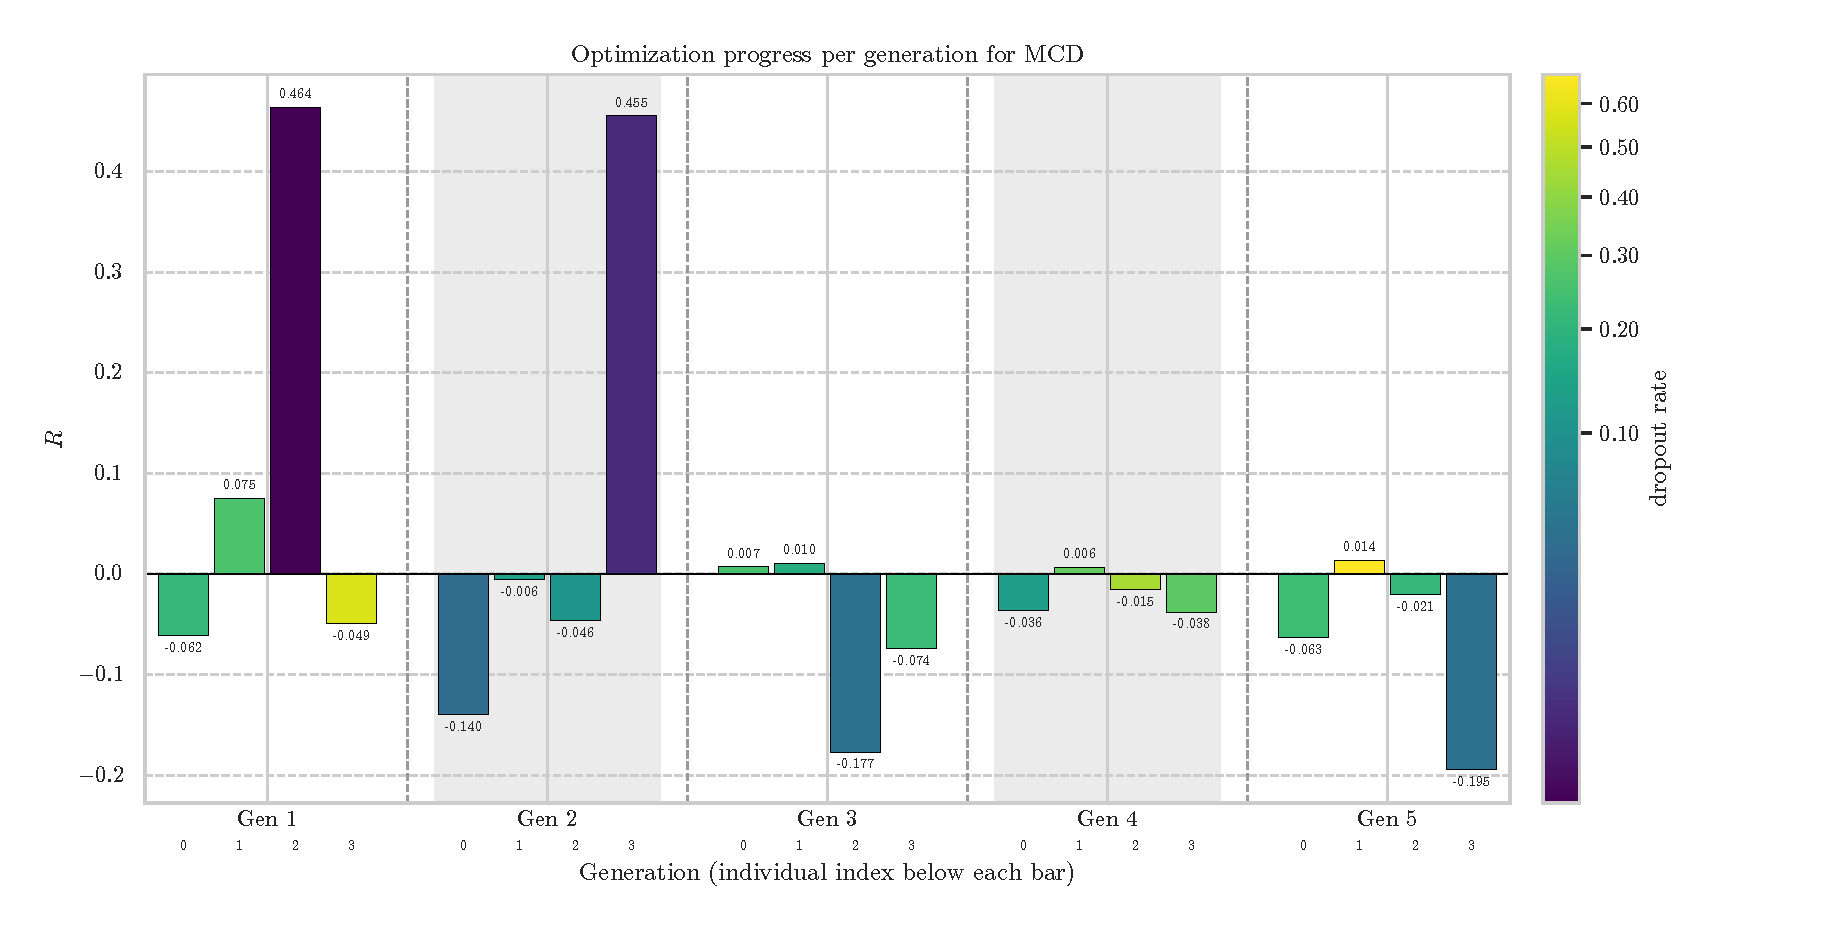
\includegraphics[width=0.9\linewidth]{imgs/mcd_evolution_history.eps}
    \caption{Evolution history of the $R$ coefficient ($R$) for the \acrshort{mcd} method.}
    \label{fig:mcd_evolution_history}
\end{figure}

\acrshort{mcd} evolution on figure \ref{fig:mcd_evolution_history} shows that the method itself is quite sensitive to hyperparameter tuning; the best performance on the calibration dataset is achieved with dropout rates $< 0.01$, beyond that, performance drops significantly and variance across populations increases dramatically, which suggests instability in the optimization process and a very narrow optimal hyperparameter range, which could be a problem for tuning this method in practice.

Best performance on the calibration dataset is achieved with a dropout rate of $\mcdRate$ and an average $R$ value of $\mcdCalibrationR$ across folds. This dropout rate is much lower than the commonly used $0.1$ or $0.2$ and is consistent with the findings of \cite{rodriguez2024uncertainty}, highlighting the importance of careful hyperparameter tuning for \acrshort{mcd}.

\begin{figure}[htbp]
    \centering
    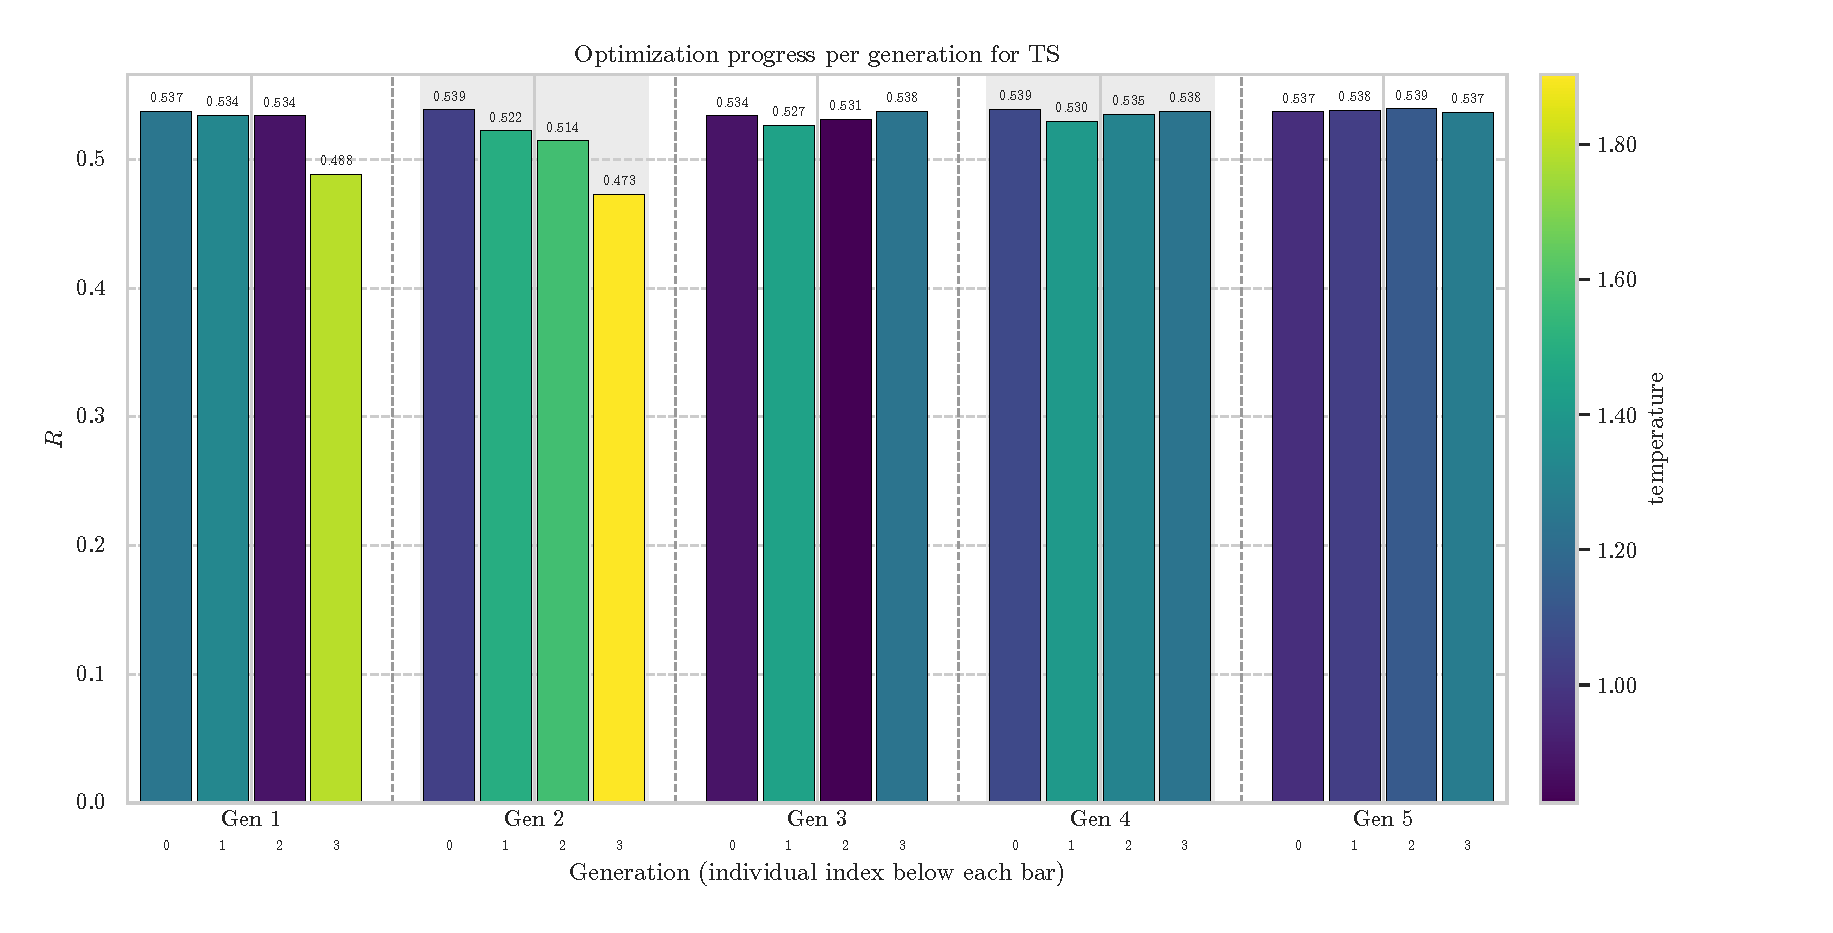
\includegraphics[width=0.9\linewidth]{imgs/ts_evolution_history.eps}
    \caption{Evolution history of the $R$ coefficient ($R$) for the \acrshort{ts} method.}
    \label{fig:ts_evolution_history}
\end{figure}

On the other hand, figure \ref{fig:ts_evolution_history} shows \acrshort{ts} is capable of providing consistent uncertainty estimates across a wide range of temperature values, with the best performance achieved around $\tau = \tsTemp$ and an average $R$ value of $\tsCalibrationR$ across folds. It's worth noting that even at the sampled extremes, performance varies less than the dropout-based methods, suggesting that \acrshort{ts} is less sensitive to hyperparameter selection in this experiment and may be a practical choice when computational resources for tuning are limited.

\begin{figure}[htbp]
    \centering
    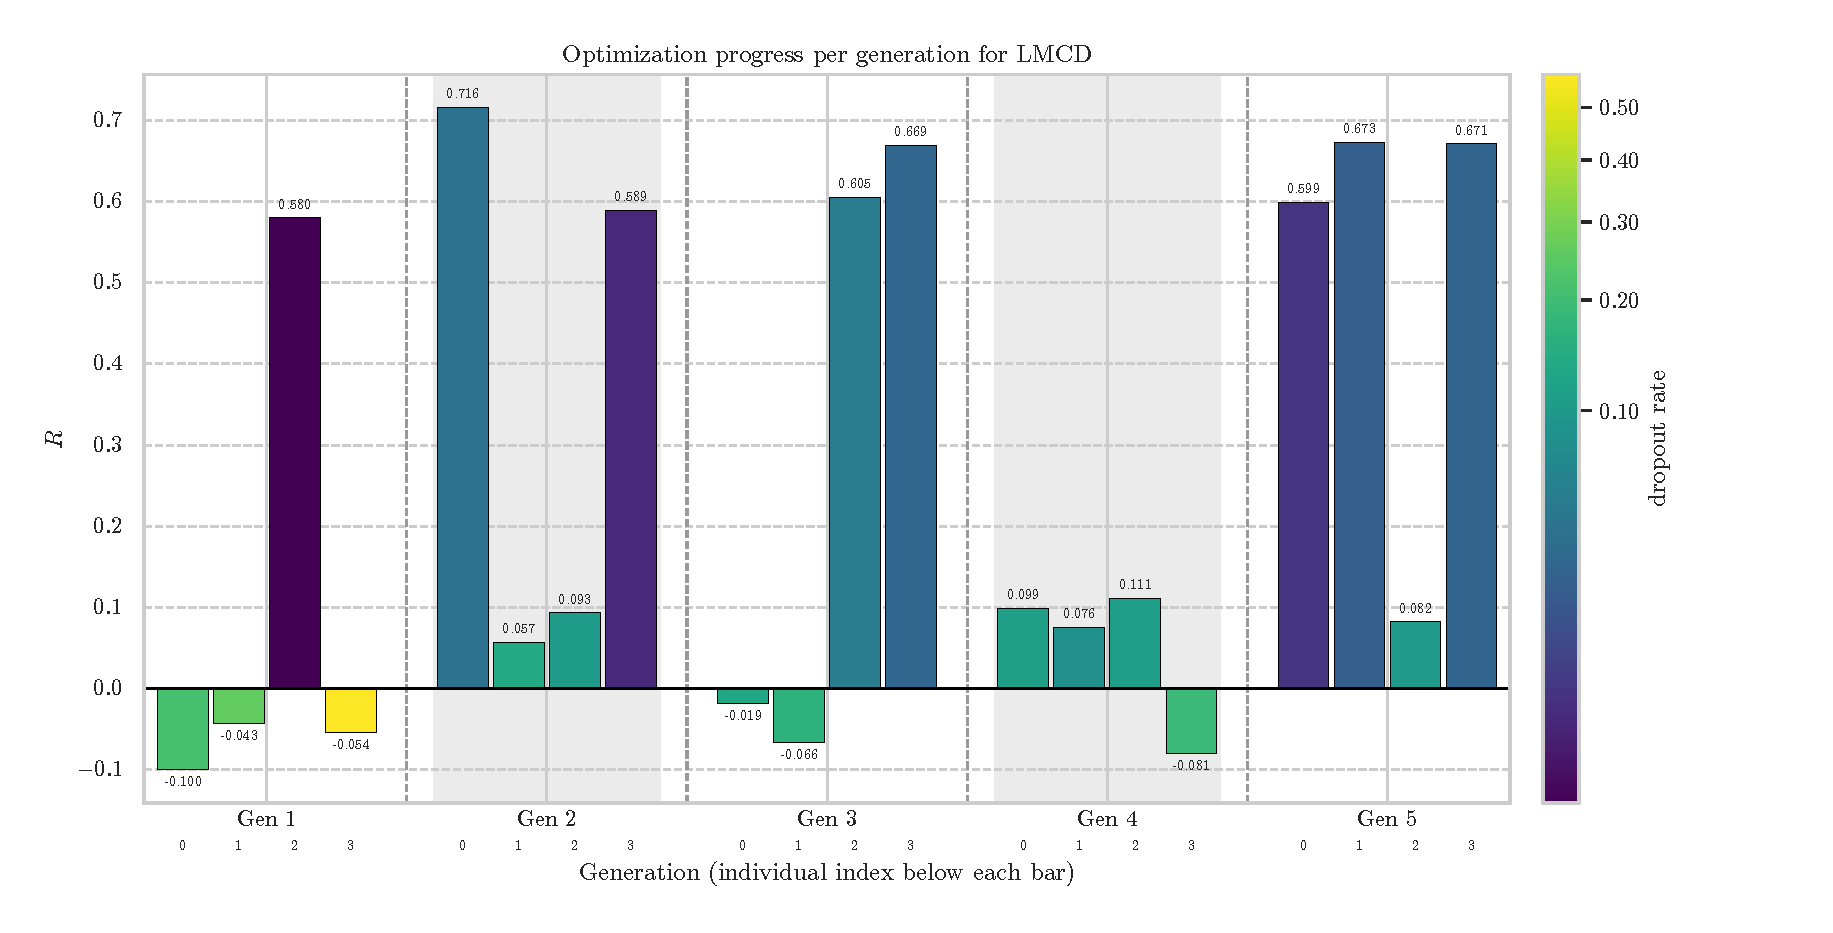
\includegraphics[width=0.9\linewidth]{imgs/lmcd_evolution_history.eps}
    \caption{Evolution history of the $R$ coefficient ($R$) for the \acrshort{lmcd} method.}
    \label{fig:lmcd_evolution_history}
\end{figure}

On figure \ref{fig:lmcd_evolution_history} \acrshort{lmcd} shows a similar pattern to \acrshort{mcd}, where lower dropout ranges provide the best performance, but manages to be more stable across a wider range of values. Best performance was achieved with a dropout rate of $\lmcdRate$ and an average $R$ value of $\lmcdCalibrationR$ across folds. \acrshort{lmcd} thus supports the trend of lower values presenting the better performance seen in \acrshort{mcd}, although this rate is an order of magnitude higher than the best rate for \acrshort{mcd}. This could be an indication that \acrshort{lmcd} is more robust to changes in the dropout rate, which could be a significant advantage in practice, as it would make the tuning process easier and less computationally expensive while providing better performance than all the other methods.


\begin{figure}[htbp]
    \centering
    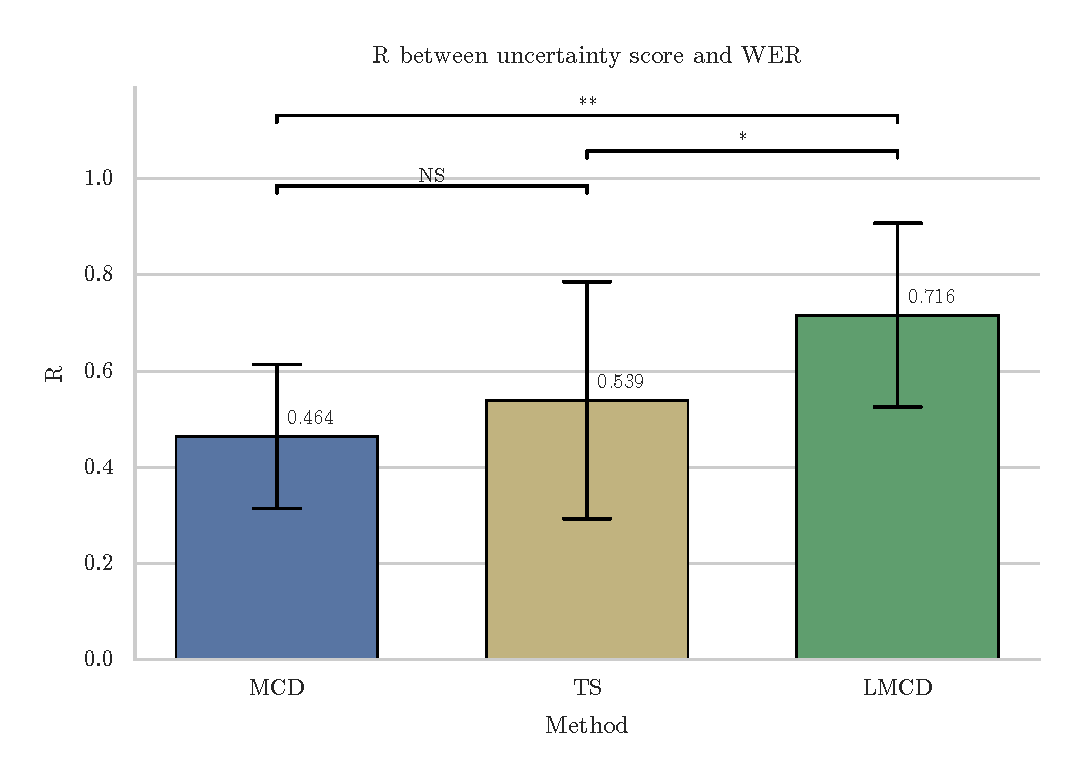
\includegraphics[width=0.9\linewidth]{imgs/best_calibration.eps}
    \caption{Best calibration results for each \acrshort{uq} method.}
    \label{fig:best_calibration_results}
\end{figure}


Table \ref{tab:wilcoxon_single_calibration} reports a one-sided Wilcoxon signed-rank test to determine whether each method's median $R$ is greater than zero across the ten folds, at $\alpha = 0.05$.
All three methods reject the null hypothesis at $p = 0.0009766$, the smallest value attainable with $N = 10$, which corresponds to every fold yielding a positive correlation. This establishes that each method produces uncertainty scores that are consistently and positively correlated with the \acrshort{wer}, but it does not by itself rank the methods; we therefore turn to a paired comparison.

Throughout the text we summarize each method by its mean $R$ across folds, whereas the tables report the median $R$ on which the test operates; the mean falls below the median for every method because one fold consistently yields a markedly lower, and for some methods slightly negative, correlation that pulls the average down.

Figure \ref{fig:best_calibration_results} summarizes the best calibration results for each \acrshort{uq} method; the whiskers represent the standard deviation of the $R$ values across folds. It also reports a paired, two-sided Wilcoxon signed-rank test between methods at $\alpha = 0.05$: \acrshort{lmcd} differs significantly from both \acrshort{mcd} ($p = 0.0020$) and \acrshort{ts} ($p = 0.027$), whereas \acrshort{mcd} and \acrshort{ts} are statistically indistinguishable ($p = 0.084$).

The advantage of \acrshort{lmcd} over \acrshort{ts} is significant but more modest than its advantage over \acrshort{mcd}, indicating that the distance-based estimation of \acrshort{lmcd} outperforms both the variance-based estimation of \acrshort{mcd} and the post-hoc calibration of \acrshort{ts}.


\begin{table}[h]
    \centering
    \begin{tabular}{|l|l|l|l|l|}
        \hline
        Method          & N  & Median & p-value   & Verdict     \\ \hline
        \acrshort{mcd}  & 10 & 0.5068 & 0.0009766 & Significant \\ \hline
        \acrshort{ts}   & 10 & 0.6634 & 0.0009766 & Significant \\ \hline
        \acrshort{lmcd} & 10 & 0.7965 & 0.0009766 & Significant \\ \hline
    \end{tabular}
    \caption{Wilcoxon signed-rank test for calibration dataset}
    \label{tab:wilcoxon_single_calibration}
\end{table}




%%%%%%%%%% Test results %%%%%%%%%%

Having defined the best hyperparameters for each method, and having validated that each one of them produces statistically significant results on the calibration dataset, we can move on to evaluate the performance of these parameters on the test dataset.

Table \ref{tab:wilcoxon_single_test} repeats the one-sided validity evaluation on the held-out test split. The null hypothesis is again rejected for every method ($p \leq 0.001953$), confirming that the positive correlation between uncertainty and \acrshort{wer} persists on data that was not used for hyperparameter selection.

\begin{table}[htbp]
    \centering
    \begin{tabular}{|l|l|l|l|l|}
        \hline
        Method & N  & Median & P value   & Verdict     \\ \hline
        MCD    & 10 & 0.4658 & 0.0009766 & Significant \\ \hline
        TS     & 10 & 0.4262 & 0.001953  & Significant \\ \hline
        LMCD   & 10 & 0.7888 & 0.001953  & Significant \\ \hline
    \end{tabular}%
    \caption{Wilcoxon signed-rank test for test dataset}
    \label{tab:wilcoxon_single_test}
\end{table}

\begin{figure}[htbp]
    \centering
    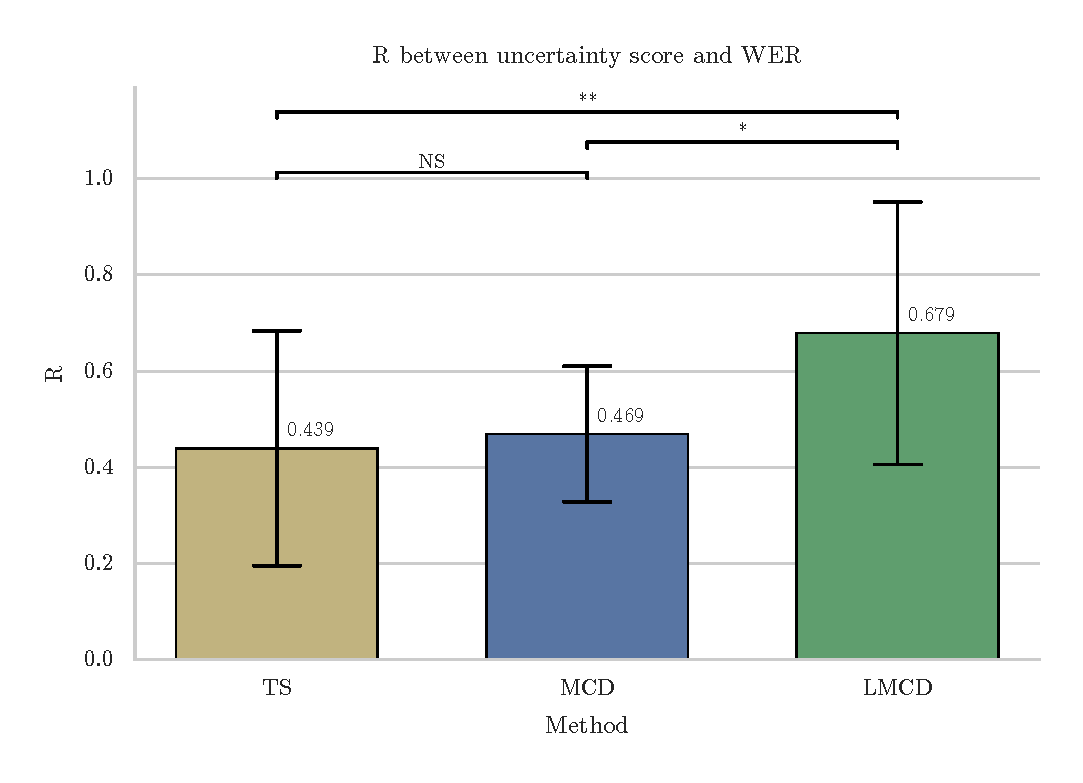
\includegraphics[width=0.9\linewidth]{imgs/best_test.eps}
    \caption{Best test results for each \acrshort{uq} method.}
    \label{fig:best_test_results}
\end{figure}


Given the validity test also holds on the test split, we again compare the methods with a paired, two-sided Wilcoxon signed-rank test; as illustrated in figure \ref{fig:best_test_results}, \acrshort{lmcd} remains significantly distinct from both \acrshort{mcd} ($p = 0.020$) and \acrshort{ts} ($p = 0.0059$), while \acrshort{mcd} and \acrshort{ts} stay statistically indistinguishable ($p = 0.49$). The ranking observed during calibration therefore carries over to the held-out data.

\begin{table}[htbp]
    \centering
    \begin{tabular}{|l|c|c|c|}
        \hline
        Method          & Optimal hyperparameter & Calibration $R$   & Test $R$   \\ \hline
        \acrshort{ts}   & $\tau = \tsTemp$       & \tsCalibrationR   & \tsTestR   \\ \hline
        \acrshort{mcd}  & dropout $= \mcdRate$   & \mcdCalibrationR  & \mcdTestR  \\ \hline
        \acrshort{lmcd} & dropout $= \lmcdRate$  & \lmcdCalibrationR & \lmcdTestR \\ \hline
    \end{tabular}
    \caption{Optimal hyperparameter and mean Pearson correlation ($R$) between the uncertainty score and \acrshort{wer}, averaged across the ten folds, for each \acrshort{uq} method on the calibration and test splits.}
    \label{tab:summary}
\end{table}

By this point, we have enough data to assert that \acrshort{lmcd} is the best method for uncertainty quantification in the tasks that we have evaluated; as summarized in Table~\ref{tab:summary}, it presents an $R$ value of $\lmcdTestR$, outperforming \acrshort{mcd} with $\mcdTestR$ and \acrshort{ts} with $\tsTestR$. It also manages to stay relatively consistent across both the calibration and test datasets, which suggests this method is more robust to changes in the data distribution, a trait that seems to be inherited from the second-place method, \acrshort{mcd}, which demonstrates robustness to changing datasets by maintaining almost the same $R$ value on both datasets.

Interestingly, \acrshort{ts} is the method that degrades the most. This is consistent with other findings such as \cite{yu2022robust}\cite{mozafari2018attended}, which show that $\tau$ is deeply tied to the data distribution used to calibrate it and is therefore more sensitive to data shift; this could become a problem in practice if the calibration set is not representative enough of the data the model will be used on.


\section{Limitations}

Several limitations bound the scope of our conclusions. First, the SpaTrans \acrshort{uq} Bench comprises roughly 66 minutes of speech across 600 short utterances; while this is sufficient to expose clear and statistically consistent differences between methods, the absolute $R$ values and optimal hyperparameters may not transfer directly to larger corpora or other domains. Second, the optimization budget was deliberately small, a population of 4 over 5 generations, i.e. 20 evaluations per method, dictated by the cost of repeated stochastic inference for the dropout-based methods; a larger budget could refine the optima, particularly for \acrshort{mcd}, whose narrow region of useful dropout values makes it sensitive to under-sampling. Third, each method exposes a single scalar hyperparameter, so our use of \acrshort{cmaes} exercises only a one-dimensional slice of its capabilities, and we did not benchmark it against other tuners such as random \cite{bergstra2012random} or Bayesian \cite{snoek2012practical} search, leaving the question of the most economical optimizer open. Fourth, our evaluation relies on Pearson correlation, which captures linear association; a strongly monotonic but non-linear relationship between uncertainty and \acrshort{wer} could be understated. Finally, all experiments use a single model (Whisper base) and a single language (Spanish), so generalization to other architectures, model sizes, and languages remains to be verified.


\section{Conclusion}

We compared three sequence-level \acrshort{uq} methods for Spanish \acrshort{asr} under a common tuning protocol, and found that \acrshort{lmcd} produces uncertainty scores that track transcription error substantially better than the established \acrshort{ts} and \acrshort{mcd} baselines. Tuning was instrumental in reaching this conclusion as it revealed that the dropout-based methods only become informative at dropout rates far below the usual $0.1$--$0.2$ defaults, underscoring how sensitive the quality of an uncertainty estimate is to a single hyperparameter.

An uncertainty score that correlates with \acrshort{wer} at $R \approx \lmcdTestR$ can be used to flag likely-erroneous transcriptions for human review, or to drive selective transcription in which only low-confidence utterances are escalated. \acrshort{lmcd} has proved to be the most capable method to do this and, like \acrshort{mcd}, it remains stable when moving from calibration to test data, whereas \acrshort{ts} degrades the most; the additional inference cost of a dropout-based method is the price for that reliability, and is justified when accurate uncertainty matters or the compute budget allows.

Several future directions follow from the limitations discussed above: validating these findings on larger corpora, additional languages, and larger Whisper variants, and exploring cheaper tuning strategies for the dropout-based methods. More broadly, the strong performance of a distance-based score suggests that sample-agreement uncertainty is a promising direction for other tasks, such as machine translation and open-ended generation.

%%
\begin{credits}
    %\subsubsection{\ackname} A bold run-in heading in small font size at the end of the paper is used for general acknowledgments, for example: This study was funded by X (grant number Y).

    \subsubsection{\discintname}
    The authors have no competing interests to declare that are
    relevant to the content of this article.
\end{credits}



%
% ---- Bibliography ----
%
% BibTeX users should specify bibliography style 'splncs04'.
% References will then be sorted and formatted in the correct style.
%
\bibliographystyle{splncs04}
\bibliography{refs}
%

\end{document}
